% Sección V: Resultados predictivos por familia de evidencia
% evidencia:E08,E09,E12,E13,E14

\section{Resultados predictivos por familia de evidencia}

Los resultados predictivos se presentan en tres bloques independientes: la corrida puntual del 18 de noviembre de 2026, los metadatos inspeccionados del artefacto cuantílico servido (\texttt{v2.0}) frente al reporte histórico del 3 de noviembre, y las dos corridas comprobadas a 120 días.

\subsection{Experimento puntual Poisson: escalera, servicios y estabilidad}

En los 26 pliegues \textit{walk-forward} reportados el 18 de noviembre de 2026~\cite{mediflow2026demanda}, incorporar estratificación por servicio, nivel local con pesos por recencia y externos aprobados reduce el error global de forma sostenida (Tabla~\ref{tab:escalera_poisson}).

\begin{table}[htbp]
\caption{Escalera predictiva puntual en 26 pliegues \textit{walk-forward} (18 de noviembre de 2026)}
\label{tab:escalera_poisson}
\centering
\scriptsize
\begin{tabularx}{\columnwidth}{@{}Y r r r r r@{}}
\toprule
Modelo evaluado & WAPE & MAE & RMSE & Sesgo & Mej. rel. \\
\midrule
1. Línea base (8 sem.) & 18,0\,\% & 77,02 & 201,34 & $+21{,}44$ & Ref. \\
2. Poisson estratificado & 15,6\,\% & 66,86 & 125,91 & $+6{,}41$ & $+13{,}2\,\%$ \\
3. LGBM nivel local (todos) & 10,5\,\% & 44,84 & 83,82 & $-6{,}00$ & $+41{,}8\,\%$ \\
4. LGBM final (\texttt{lgbm\_final}) & 10,5\,\% & 44,94 & 83,67 & $-5{,}70$ & $+41{,}6\,\%$ \\
\bottomrule
\end{tabularx}
\ieeenota{Datos archivados de~\cite{mediflow2026demanda} (sec.~1, orígenes \texttt{2025-07-25} a \texttt{2026-07-10}, horizonte 1--7\,d, sin \texttt{Otros}). Las mejoras relativas fueron calculadas con cifras sin redondear. \texttt{lgbm\_final} conserva solo \texttt{festivos\_y\_puentes} y \texttt{carnaval\_y\_semana\_santa}.}
\end{table}

El desempeño desagregado de \texttt{lgbm\_final} muestra marcada heterogeneidad (Tabla~\ref{tab:servicios_poisson}). Urgencias (\texttt{9203}) y Rehabilitación (\texttt{581479}) obtienen WAPE de 8,4\,\% y 11,0\,\% (exactitudes $1-\text{WAPE}$ de 91,6\,\% y 89,0\,\%); sin embargo, en Rehabilitación la exactitud cae a 51,3\,\% los sábados (87,1 llegadas/día) y 15,6\,\% los domingos (2,2/día), frente a 85,6\,\%--90,9\,\% de lunes a viernes (835,7--1.306,2/día)~\cite{mediflow2026demanda}. En Tratamiento Urgencias (\texttt{3045729}, media 15,17/día), el WAPE diario alcanza 43,5\,\% (exactitud 56,5\,\%, MAE 6,59), frente a un techo Poisson idealizado de 79,5\,\% diario; al agregar la semana completa alcanza 77,0\,\% frente a un techo semanal de 92,3\,\%~\cite{mediflow2026demanda}. Al quedar bajo ambas cotas, influyen tanto la varianza de conteos bajos como cambios semanales de tasa.

\begin{table}[htbp]
\caption{Desempeño por servicio del experimento puntual \texttt{lgbm\_final}}
\label{tab:servicios_poisson}
\centering
\scriptsize
\begin{tabularx}{\columnwidth}{@{}Y r r r r r@{}}
\toprule
Servicio & WAPE & $1-\text{WAPE}$ & MAE & Sesgo & Prom. \\
\midrule
Urgencias (\texttt{9203}) & 8,4\,\% & 91,6\,\% & 37,02 & $-7{,}83$ & 443,16 \\
Rehabilitación (\texttt{581479}) & 11,0\,\% & 89,0\,\% & 91,22 & $-10{,}12$ & 826,54 \\
Trat. Urgencias (\texttt{3045729}) & 43,5\,\% & 56,5\,\% & 6,59 & $+0{,}86$ & 15,17 \\
\bottomrule
\end{tabularx}
\ieeenota{Datos archivados de~\cite{mediflow2026demanda} (sec.~2, 26 pliegues, 182 días/servicio, sin \texttt{Otros}). No transferir estas cifras al modelo cuantílico web.}
\end{table}

En días normales, el WAPE baja de 12,4\,\% en línea base (MAE 55,63; sesgo $-3{,}45$) a 10,3\,\% en \texttt{lgbm\_final} (MAE 45,97; sesgo $-6{,}96$); en festivos, cae de 317,8\,\% (MAE 409,64; sesgo $+408{,}36$, por sobreestimación en cierres de Rehabilitación) a 22,5\,\% (MAE 29,03; sesgo $+13{,}89$)~\cite{mediflow2026demanda}. A lo largo del horizonte 1--7 días, el WAPE oscila entre 9,4\,\% (día 7, jueves) y 17,0\,\% (día 2, sábado), y entre pliegues va de 5,4\,\% (pliegue 17, \texttt{2026-03-20}) a 28,0\,\% en el pliegue 11 (\texttt{2025-12-26}, fin de año; línea base 137,9\,\%) y 27,6\,\% en el pliegue 19 (\texttt{2026-04-17})~\cite{mediflow2026demanda} (detalle completo en Anexo~B).

\subsection{Artefacto cuantílico servido en la aplicación web (\texttt{v2.0})}

Los metadatos inspeccionados directamente en \texttt{models/modelos\_web\_bundle.joblib} (\texttt{comparacion\_real} sobre 182 días, \texttt{2025-07-25} a \texttt{2026-07-16}) reportan el rendimiento del modelo cuantílico $p_{10}/p_{50}/p_{90}$ servido por la API (Tabla~\ref{tab:bundle_cuantilico}). El WAPE de $p_{50}$ es 8,91\,\% en Urgencias, 11,08\,\% en Rehabilitación y 42,18\,\% en Tratamiento Urgencias; las coberturas $p_{10}$--$p_{90}$ (78,57\,\%, 64,29\,\% y 73,08\,\%) quedan por debajo de 80\,\%, especialmente en Rehabilitación por sus cierres bruscos y la ausencia de nivel local.

\begin{table*}[t]
\caption{Métricas archivadas del modelo cuantílico servido en el artefacto web \texttt{v2.0}}
\label{tab:bundle_cuantilico}
\centering
\footnotesize
\begin{tabularx}{\textwidth}{@{}Y r r r r r r@{}}
\toprule
Servicio en bundle \texttt{v2.0} & WAPE & MAE & RMSE & Sesgo & Cob. $p_{10}$--$p_{90}$ & Exact. sem. \\
\midrule
Urgencias (\texttt{9203}) & 8,91\,\% & 39,50 & 53,82 & $-2{,}69$ & 78,57\,\% & 94,75\,\% \\
Rehabilitación (\texttt{581479}) & 11,08\,\% & 91,55 & 137,57 & $+4{,}22$ & 64,29\,\% & 91,63\,\% \\
Tratamiento Urg. (\texttt{3045729}) & 42,18\,\% & 6,40 & 8,47 & $-0{,}64$ & 73,08\,\% & 76,60\,\% \\
\bottomrule
\end{tabularx}
\ieeenota{Metadatos de \texttt{comparacion\_real} en~\cite{mediflow2026bundle} (182 días: \texttt{2025-07-25} a \texttt{2026-07-16}, corte exclusivo \texttt{2026-07-17}; vía \texttt{GET /api/modelo}). Cobertura calculada antes de redondear puntos a enteros. Techos Poisson almacenados: Urgencias 96,21\,\% diario / 98,57\,\% semanal; Rehabilitación 97,22\,\% / 98,95\,\%; Tratamiento Urgencias 79,53\,\% / 92,26\,\%.}
\end{table*}

Estas cifras no deben confundirse con el reporte histórico del 3 de noviembre de 2026~\cite{mediflow2026intervalos}, que documentó cobertura global de 83,2\,\% (85,2\,\% en Urgencias, 72,0\,\% en Rehabilitación, 75,8\,\% en Tratamiento y 100,0\,\% en \texttt{Otros}; amplitud media 112,6 pacientes) sobre una versión previa e incluyendo \texttt{Otros}. Además, al consultar fechas futuras sin rezagos observados, \texttt{predict.py} usa \texttt{medianas\_dw}, lo cual no replica las condiciones del backtest 1--7 días. La Fig.~\ref{fig:resumen_escalera} separa visualmente el experimento puntual de la simulación de altas tempranas.

\begin{figure*}[t]
\centering
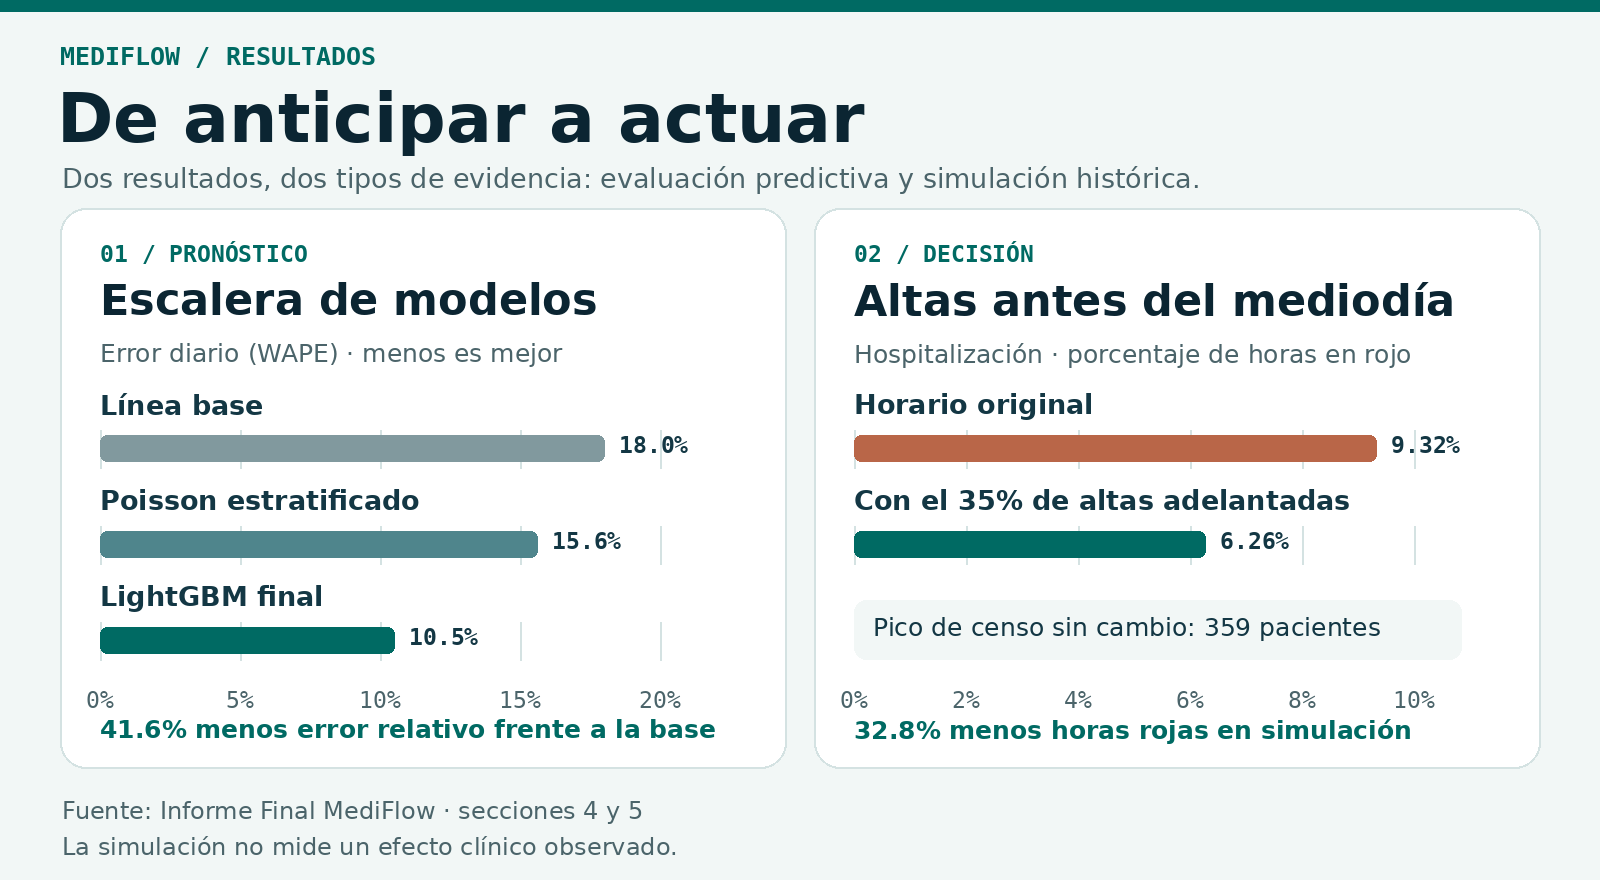
\includegraphics[width=0.84\textwidth]{resumen_escalera_optimizacion.png}
\caption{Síntesis comparativa entre evaluación predictiva puntual y simulación histórica de altas (\texttt{resumen\_escalera\_optimizacion.png}). Panel izquierdo: experimento puntual Poisson en 26 pliegues (no modelo cuantílico web). Panel derecho: simulación determinista de adelanto del 35\,\% de altas en Hospitalización (no ensayo clínico).}
\label{fig:resumen_escalera}
\end{figure*}

\subsection{Horizonte extendido a cuatro meses: reporte histórico frente a bundle}

Se documenta por separado la divergencia entre el reporte histórico del 3 de noviembre de 2026~\cite{mediflow2026largoplazo} y el campo \texttt{largo\_plazo} inspeccionado en el bundle \texttt{v2.0}~\cite{mediflow2026bundle} (Tabla~\ref{tab:largo_plazo_comparado}). En~\cite{mediflow2026largoplazo}, la exactitud global cae de 87,8\,\% en el mes 1 (WAPE 12,2\,\%) a 86,6\,\% (13,4\,\%), 83,5\,\% (16,5\,\%) y 78,7\,\% en el mes 4 (WAPE 21,3\,\%, ancho medio 424,5 pacientes), con 50,7\,\% de exactitud semanal (WAPE 49,3\,\%) en Tratamiento Urgencias. En el bundle \texttt{v2.0}, las tres series muestran menor WAPE y proyecciones agosto--noviembre coherentes con los niveles recientes de mediados de 2026 (frente a los promedios menores de la corrida del 3 de noviembre), aunque Rehabilitación cae bajo 80\,\% de cobertura en el mes 1 (77,69\,\%). El desglose mensual completo figura en el Anexo~B.

\begin{table*}[t]
\caption{Desempeño del modelo de largo plazo (120 días, 13 pliegues): reporte archivado frente a bundle servido}
\label{tab:largo_plazo_comparado}
\centering
\footnotesize
\begin{tabularx}{\textwidth}{@{}L{0.25\textwidth} Y r r r r r@{}}
\toprule
Fuente y corrida & Servicio & WAPE & $1-\text{WAPE}$ & MAE & Sesgo & Cobertura \\
\midrule
Reporte archivado & Global (sin \texttt{Otros}) & 15,7\,\% & 84,3\,\% & 57,9 & --- & 86,5\,\% \\
(\texttt{2026-11-03})~\cite{mediflow2026largoplazo} & Urgencias (\texttt{9203}) & 14,0\,\% & 86,0\,\% & 52,3 & $+20{,}1$ & 85,4\,\% \\
 & Rehabilitación (\texttt{581479}) & 15,5\,\% & 84,5\,\% & 111,7 & $+44{,}2$ & 85,3\,\% \\
 & Tratamiento (\texttt{3045729}) & 64,4\,\% & 35,6\,\% & 9,8 & $+4{,}9$ & 88,7\,\% \\
\midrule
Bundle servido \texttt{v2.0} & Urgencias (\texttt{9203}) & 11,63\,\% & 88,4\,\% & 51,8 & $-15{,}1$ & 87,18\,\% \\
(inspección \texttt{2026-11-19})~\cite{mediflow2026bundle} & Rehabilitación (\texttt{581479}) & 14,33\,\% & 85,7\,\% & 122,7 & $-2{,}9$ & 83,40\,\% \\
 & Tratamiento (\texttt{3045729}) & 58,12\,\% & 41,9\,\% & 10,1 & $+3{,}9$ & 88,65\,\% \\
\bottomrule
\end{tabularx}
\ieeenota{Dos corridas independientes sobre 13 pliegues solapados (\texttt{2025-03-24} a \texttt{2026-03-19}). En~\cite{mediflow2026largoplazo} las proyecciones ago--nov 2026 promedian 215,7--221,0/d (Urgencias) y 330,5--385,9/d (Rehabilitación); en~\cite{mediflow2026bundle}, promedian 415,6--433,2/d (Urgencias), 661,5--789,6/d (Rehabilitación, cobertura 77,69\,\% mes 1 y 81,79\,\%--87,95\,\% meses 2--4) y 15,6--16,1/d (Tratamiento). Son extrapolaciones desde el corte de julio de 2026, no demanda real observada.}
\end{table*}
